\documentclass[]{article}
\usepackage{amsmath}
\usepackage{amsfonts}
\usepackage{amssymb}
\usepackage{algorithmic}
\usepackage{algorithm}
\usepackage{tikz}
\usepackage{graphicx}
\usepackage{mdframed}
\usepackage{paralist}
\usepackage{listings}

\definecolor{dkgreen}{rgb}{0,0.6,0}
\definecolor{gray}{rgb}{0.5,0.5,0.5}

\lstset{
  language=Python,
  breaklines=true,
  showstringspaces=false,
  frame=single,
  aboveskip=3mm,
  belowskip=3mm,
  columns=flexible,
  basicstyle={\small\ttfamily},
  numbers=none,
  numberstyle=\tiny\color{gray},
  keywordstyle=\color{blue},
  commentstyle=\color{gray},
  stringstyle=\color{dkgreen},
  breakatwhitespace=true,
  tabsize=3
}

\title{CAGD - Homework 2}
\author{Josefine St{\aa}l \& Erik Ackzell}

\begin{document}

\maketitle
\section*{Task 1}
In this task we implement subdivision to split a B\'ezier curve into two different B\'ezier curves. This is implemented as a method of a Python class, see Appendix 1. Details can be seen in the code. We then test our code by defining a B\'ezier curve with control points $(-1, 0), (0, 1), (2, 0)$, subdividing at $t=0.4$. In our test, the control points of the two new B\'ezier curves were $(-1, 0), (-0.6, 0.4), (-0.04, 0.48)$ and $(-0.04, 0.48), (0.8, 0.6), (2, 0)$. The original curve can be seen in the figure below.
\begin{figure}[h!]
	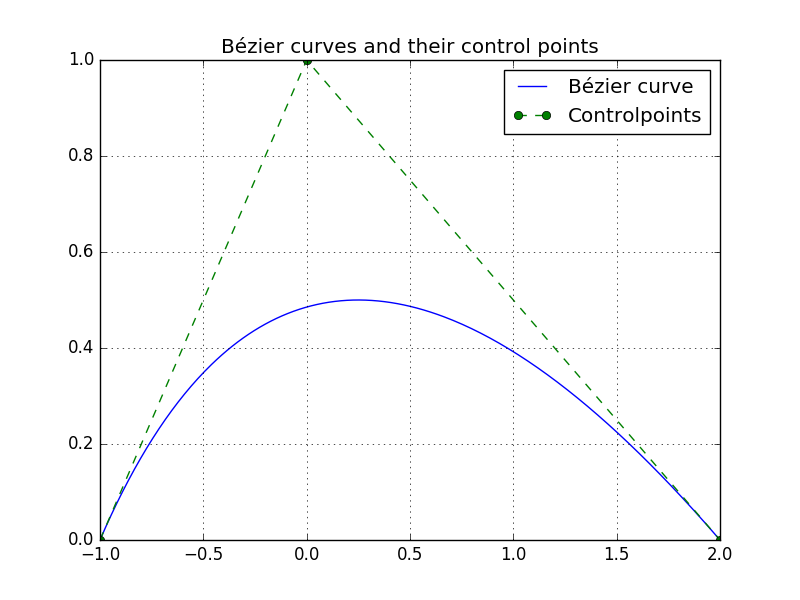
\includegraphics[scale=0.6]{beziercurvefig}
\end{figure}

\section*{Task 2}
In this task we implement degree elevation for the B\'ezier curve with the same control points as in task 1. This is implemented as a method of a Python class, see Appendix 1. Details can be seen in the code. In our test, the control points of the B\'ezier curve from task 1 were used, and the degree was increased to four. The control points of the new curve were $(-1, 0), (-0.5, 0.5), (0.17, 0.7), (1, 0.5), (2, 0)$.

\section*{Task 3}
In this task, we used the trivial reject approach in order to determine the intersection of a B\'ezier curve and a line. This is implemented as a method of a Python class along with a rectangle class and a line class, see Appendix 1. Details can be seen in the code. In our test, we used the B\'ezier curve with control points $(0, 0), (9, -4), (7, 5), (2, -4)$ and the line passing through $(4, 5)$ and $(6, -4)$. The intersections found were $(5.32, -0.94)$ and $(5.13, -0.10)$.

\section*{Task 6}
In this task, we change the appearance of a curve (top curve in figure below to the lower curve) by adding one more control point. The control points of the original curve is given by $(0, 0), (1, 1), (2, 1)$ and the second curve has control points $(0, 0), (0.25, 0.05), (1, 1), (2, 1)$.

\begin{figure}[h!]
	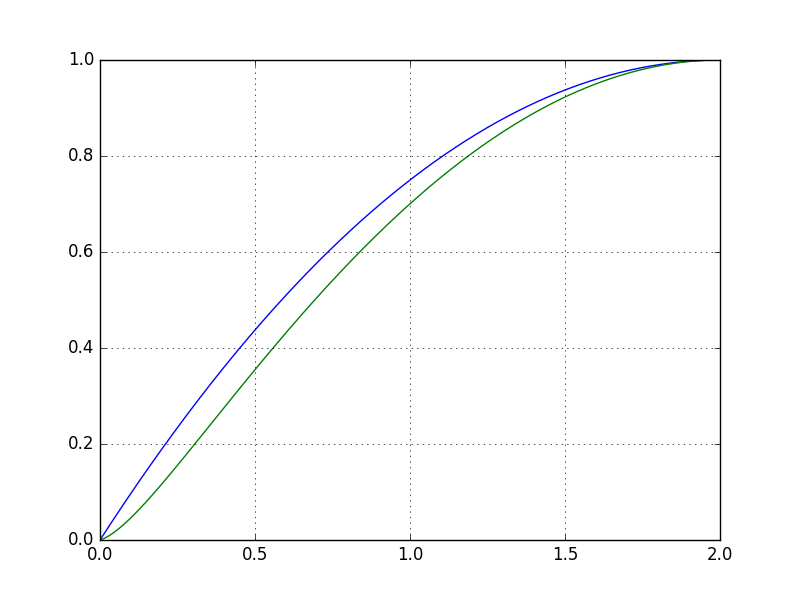
\includegraphics[scale=0.6]{non_symmetric_degree_elevation}
\end{figure}

\newpage
\section*{Appendix I}
Code for task 1-3.
\lstinputlisting[lastline=347]{beziercurveclass.py}

\end{document}
